\documentclass[10pt]{article}
\usepackage[paperwidth=8.5in,paperheight=11in,left=0.9in,right=0.9in,top=0.85in,bottom=0.9in]{geometry}
\usepackage{multicol}
\usepackage{mathptmx}
\usepackage{amsmath,amssymb}
\usepackage{graphicx}
\usepackage{booktabs}
\usepackage{float}
\usepackage{caption}
\usepackage{titlesec}
\usepackage{fancyhdr}
\usepackage{tikz}
\usetikzlibrary{arrows.meta,positioning}
\usepackage[hidelinks]{hyperref}

\captionsetup{font=small,labelfont=sc,labelsep=period,justification=justified,singlelinecheck=false,skip=4pt}
\renewcommand{\figurename}{FIG.}
\renewcommand{\tablename}{TABLE}
\renewcommand{\thetable}{\Roman{table}}
\newcommand{\secnum}{\Roman{section}}
\titleformat{\section}{\normalfont\bfseries\large}{\secnum.}{0.6em}{\MakeUppercase}
\titleformat{\subsection}{\normalfont\bfseries\itshape}{\Alph{subsection}.}{0.5em}{}
\titlespacing{\section}{0pt}{1.2ex plus .3ex}{0.6ex}
\titlespacing{\subsection}{0pt}{0.9ex plus .2ex}{0.4ex}
\setlength{\columnsep}{0.28in}
\setlength{\parskip}{0pt}
\setlength{\parindent}{10pt}
\renewcommand{\baselinestretch}{0.97}
\pagestyle{fancy}
\fancyhf{}
\fancyhead[C]{\thepage}
\renewcommand{\headrulewidth}{0pt}

\newcommand{\All}{\ensuremath{\mathrm{AllParticles}}}
\newcommand{\Perf}{\ensuremath{\mathrm{PerfectReco}}}
\newcommand{\eff}{\ensuremath{\varepsilon}}

\begin{document}

\begin{center}
{\LARGE\bfseries Bug fixes and pruning optimization for\\[2pt] inclusive beauty-hadron reconstruction\par}
\vspace{0.9em}
{\large Q.~Guo\par}
\vspace{0.35em}
{\small University of Chinese Academy of Sciences, Beijing 100049, China\par}
\end{center}

\vspace{0.3em}
\begin{center}
\begin{minipage}{0.86\textwidth}
\textbf{Abstract.} Reconstruction of beauty-hadron decays at the LHCb upgrade must run in real time on events with up to a thousand charged tracks. Deep full event interpretation (DFEI) represents an event as a graph of track pairs, prunes the graph with two graph neural networks, classifies each surviving pair by its lowest common ancestor generation (LCAG), and assembles decay chains from the classified graph. We measure the effect of five changes to the pruning stage, one at a time. On a simulated inclusive $b\bar b$ sample with a fixed denominator of 13\,255 signal chains, moving the cut on the pruning scores raises the efficiency from 14.5\% to 17.9\% without retraining. A pairwise ranking term, matched to the thresholded use of the score, adds 2.6 points at the new working point. Three features computed from the two track trajectories raise the intermediate 22.6\% model to 26.0\%; six edge-context inputs and one round of attention on the line graph add 1.0 point each, the latter only when the pair geometry enters the attention logits. The efficiency reaches 28.0\%. All numbers are single-variable effects measured on one simulated sample; the statistical resolution is 0.4 points and no training variance is included.
\end{minipage}
\end{center}

\vspace{0.5em}
\begin{multicols}{2}

\section{Introduction}

The LHCb experiment will operate at a luminosity ten times the design value in Upgrade II, with up to fifty proton-proton collisions per bunch crossing and a charged-track multiplicity of order $10^3$ per event \cite{upgrade2}. Storing every event is not possible, and selecting events by reconstructing predefined candidates does not scale to the tens of thousands of decay modes of interest. Inclusive strategies instead interpret the event as a whole and retain the parts that belong to a heavy-flavour decay.

Deep full event interpretation (DFEI) is one such strategy \cite{dfei,hgnn}. Charged tracks are the nodes of a graph and every pair of tracks is a candidate edge. A node-pruning network removes tracks that are inconsistent with a $b$-hadron decay; an edge-pruning network removes pairs that are unlikely to belong to the same decay chain; a third network assigns each surviving pair an LCAG class, which encodes the generation of the shared ancestor for classes 0--3. Chains are defined as the connected components of the pairs with LCAG $>0$ (Fig.~\ref{fig:pipe}).

\begin{figure}[H]
\centering
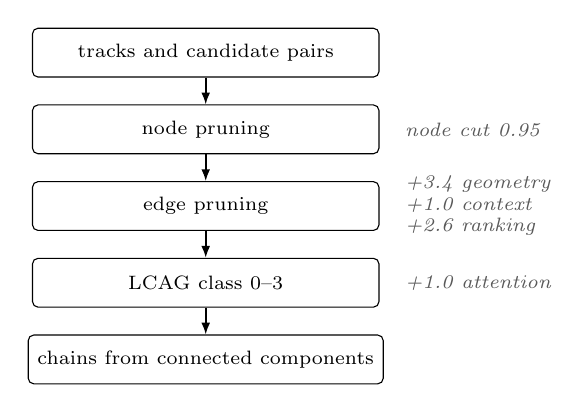
\begin{tikzpicture}[font=\scriptsize, node distance=3.4mm,
  box/.style={draw, rounded corners=2pt, minimum width=4.4cm, minimum height=6.2mm, align=center, fill=white},
  lab/.style={font=\scriptsize\itshape, text=black!65, align=left},
  arr/.style={-{Latex[length=1.5mm]}, semithick}]
\node[box] (a) {tracks and candidate pairs};
\node[box, below=of a] (b) {node pruning};
\node[box, below=of b] (c) {edge pruning};
\node[box, below=of c] (d) {LCAG class 0--3};
\node[box, below=of d] (e) {chains from connected components};
\draw[arr] (a)--(b); \draw[arr] (b)--(c); \draw[arr] (c)--(d); \draw[arr] (d)--(e);
\node[lab, right=2mm of b] {node cut 0.95};
\node[lab, right=2mm of c, align=left] {+3.4 geometry\\+1.0 context\\+2.6 ranking};
\node[lab, right=2mm of d] {+1.0 attention};
\node[lab, right=2mm of e] {};
\end{tikzpicture}
\caption{Pipeline of DFEI and the places where this work adds information. The numbers are single-variable gains in percentage points of the fixed denominator and are not additive.}
\label{fig:pipe}
\end{figure}

This paper reports where the chain efficiency is lost in that pipeline and what has to be added to move it. The study uses a simulated inclusive $b\bar b$ sample, referred to below as the 0904 sample, with a fixed denominator of 13\,255 signal chains in a sample of 20\,000 simulated events. Throughout we quote efficiencies, not event yields. \All{} is the fraction of signal chains whose reconstructed cluster contains exactly the truth tracks and no others; \Perf{} additionally requires the LCAG values of all pairs inside the cluster to agree with the truth. Both are quoted in percent of the fixed denominator. The binomial error from this denominator is $\pm0.4$ percentage points at the 28\% level for a single number, and $\pm0.5$ for the difference of two independent runs; training variance is not included, since all entries are single runs.

The paper is organised as follows. Section~\ref{sec:pipeline} describes the pipeline, the sample and the metrics. Section~\ref{sec:changes} introduces the five changes and gives the corresponding measurements one at a time. Section~\ref{sec:results} collects the cumulative effect, the global ranking and the score distributions. Section~\ref{sec:discussion} discusses the attribution and the limitations. Three appendices contain the DOCA sign error, the PV-association result, and the definitions of the small changes.

\section{The DFEI pipeline}
\label{sec:pipeline}

\subsection{Graph construction and pruning}

An event is represented by a heterogeneous graph with tracks and primary vertices (PVs) as node types. Track nodes carry kinematic and impact-parameter information and the associated PV. A track pair carries kinematic inputs ($\Delta R$, $\Delta z$, the sum of charges, $\Delta p_T$), impact-parameter inputs ($\Delta$IP and a rank variable), the distance of closest approach (DOCA) and derived quantities including a triangle-transitivity term built from a third track.

A node-pruning MLP scores each track and an edge-pruning MLP scores each pair. A pair is kept when both scores exceed their thresholds. The surviving pairs are classified into LCAG 0--3, and chains are the connected components of the pairs with a positive class. The baseline uses a threshold of 0.90 on both scores and a binary cross-entropy whose positive weight is about 800, reflecting the signal fraction of roughly 0.13\% among candidate pairs. Models are trained with Adam, a batch size of eight, a learning rate of $10^{-4}$ and 20 epochs (early stopping on the validation loss). The backbone has four graph blocks with 128--128--16 MLPs and a 16-dimensional latent space. Thresholds and model versions are compared on the same sample and with the same denominator throughout.

\subsection{Dataset and metrics}

The 0904 sample is a simulated inclusive $b\bar b$ sample. The test set contains 20\,000 simulated events and 13\,255 signal chains. A signal chain is a truth $b$-hadron decay chain; a reconstructed cluster is accepted by \All{} when it contains exactly the tracks of one truth chain and no others. \Perf{} additionally requires the LCAG class of every pair inside the cluster to agree with the truth. All efficiencies are quoted as a fraction of the fixed denominator, so that a change in the number of accepted clusters cannot change the normalisation and two versions can be compared directly.

\subsection{Previous round and PV association}

An earlier round on a different production sample moved the GNN side of the pipeline from 22.5\% to 36.7\% and then saturated. That sample is not comparable with the 0904 sample, and no number from it is used below; it motivates moving from the network architecture to the pruning inputs. The same round also addressed PV association: four models trained on a sample with leakage give 13.1--14.0\% misassociation on corrected data (average 13.6\%), models retrained on the corrected sample give 8.6\%, and the minIP baseline gives 10.15\%. The retrained model also uses an auxiliary PV head, and the two changes were introduced together, so the difference cannot be attributed to the head alone. Details and the corresponding figure are given in Appendix~\ref{app:pv}.

\section{Changes to the pruning stage}
\label{sec:changes}

\subsection{The cut on the pruning scores}

The first change is not a model change. The baseline weights are kept and the cut on the node and edge scores moves from 0.90 to 0.95; at 0.97 the efficiency is 18.5\%, but the later comparisons use 0.95. Figure~\ref{fig:thr} shows the three points. At 0.90, 0.95 and 0.97 the values of \All{} are 14.5\%, 17.9\% and 18.5\%, and those of \Perf{} are 9.5\%, 11.7\% and 11.9\%. The gain of 3.4 points at 0.95 therefore involves no retraining: it is a choice of where to cut, and all numbers below use 0.95.

\begin{figure}[H]
\centering
\includegraphics[width=\columnwidth]{figs/thr.png}
\caption{\All{} (left bar of each pair) and \Perf{} (right bar) for the baseline weights at three cuts on the pruning scores. No retraining is involved.}
\label{fig:thr}
\end{figure}

Because the working point is a hyperparameter, the gain is realised only if the cut can be calibrated on data. For a trigger this would require a dedicated control sample; the quoted value is therefore an upper bound for a trigger application, and the comparison with model changes should be read with that caveat.

\subsection{Vertex geometry}

The two DOCA features are recomputed from the track states. The stored column comes from an expression with a sign error, described in Appendix~\ref{app:doca}; it is not symmetric under exchange of the two tracks, and its correlation with the recomputed value is 0.019, so it behaves as noise. The third feature, $|\Delta \mathrm{start}|$, is a new absolute quantity: the older derived block contained only $d_\perp/(|\Delta z|+1)$, which removes the overall scale. The three features are $\mathrm{DOCA}/100$, $\log(\mathrm{DOCA})$ and $|\Delta \mathrm{start}|/100$, with distances in mm.

With the three features the efficiency moves from 22.6\% to 26.0\% and \Perf{} from 14.8\% to 17.8\% (Fig.~\ref{fig:vertex}). The three features enter together, so the gain cannot be split further; there is no run with $|\Delta \mathrm{start}|$ alone. Whether replacing the stored column alone would help cannot be isolated from the archived runs: the only run with the corrected column also adds the other derived inputs, so the two are confounded.

\begin{figure}[H]
\centering
\includegraphics[width=0.92\columnwidth]{figs/doca.png}
\caption{\All{} and \Perf{} before and after the three vertex-geometry features are added to the 22.6\% model.}
\label{fig:vertex}
\end{figure}

\subsection{Pairwise ranking term}

The positive weight of the BCE lifts signal edges but leaves their order against a background edge unconstrained, while the reconstruction thresholds the score. A pairwise term is added for this reason: every signal edge is compared with the 64 highest-scoring background edges of the same event,
\begin{equation}
L_{\mathrm{rank}}=\big\langle \max(0,\ \tau+s_{\mathrm{bkg}}-s_{\mathrm{sig}})\big\rangle,\qquad \tau=1,
\label{eq:rank}
\end{equation}
with weight 10 in $L=L_{\mathrm{BCE}}+10\,L_{\mathrm{rank}}$. Here $s$ denotes the pruning logit, which is unbounded, so $\tau$ is a margin in logit units. At the original cut the term changes \All{} from 14.5\% to 16.3\%, and at 0.95 from 17.9\% to 20.5\%; \Perf{} changes from 9.5\% to 11.1\% and from 11.7\% to 13.6\% (Fig.~\ref{fig:rank}). Since only the relative order enters, the absolute score drifts and the working point has to be re-scanned; the two points shown in the figure are measured after that re-scan.

\begin{figure}[H]
\centering
\includegraphics[width=\columnwidth]{figs/rankeff.png}
\caption{\All{} at two working points, with and without the pairwise ranking term. The threshold is re-scanned in both cases.}
\label{fig:rank}
\end{figure}

\subsection{Edge-context inputs}

The pair representation is extended with six inputs that summarise the other candidate pairs attached to the two tracks. Let $C(t)$ be the set of candidate pairs attached to track $t$; a pair $e=(i,j)$ belongs to both $C(i)$ and $C(j)$. With $d_3$ the distance between the two production vertices in mm and $A=\exp(-d_3/50)$, one defines at each end
\begin{equation}
\begin{aligned}
r_t&=\frac{A_e}{\max_{f\in C(t)}A_f},\quad
d_t=\frac{\#\{f\in C(t): A_f>0.5\}}{10},\\
c_t&=\frac{|C(t)|}{50}.
\end{aligned}
\label{eq:ctx}
\end{equation}
The six inputs are the minimum and maximum of $r$, $d$ and $c$ over the two ends, which makes the vector symmetric under exchange of $i$ and $j$; the mother-daughter direction is not reliable at this stage. The constants are fixed heuristics and were not tuned; the threshold $A>0.5$ corresponds to a separation of about 35~mm, which is several times the typical flight distance of a $b$ hadron, so the affinity varies slowly across the candidates of one track. The two counts differ: $d$ counts only pairs with $A>0.5$, whereas $c$ counts all candidates of the track. The adapter that carries the new inputs is zero-initialised, so the previous model is recovered at initialisation.

With the six inputs the efficiency moves from 26.0\% to 27.0\% (Fig.~\ref{fig:ctx}). At 0.90, where the comparison with the previous step is made, the number of retained background edges falls by 16\% while the number of retained signal edges falls by 3\%, so the purity of the kept edges rises from 11.6\% to 13.1\%. The global average precision of the edge score falls from 0.325 to 0.314: the gain is concentrated on nearly degenerate pairs, the region that determines whether a chain survives, whereas the global average is dominated by easily separated pairs.

\begin{figure}[H]
\centering
\includegraphics[width=\columnwidth]{figs/dist_m2.png}
\caption{Edge-score distribution before (left) and after (right) the edge-context inputs, for background (grey) and signal (green) pairs. The vertical line marks the 0.90 cut.}
\label{fig:ctx}
\end{figure}

\subsection{Attention on the line graph}

Candidate pairs become the nodes of a line graph, and two pairs are neighbours when they share a track in the same event; the neighbourhood is truncated to at most 32 pairs per shared track, selected by representation norm. One round of four-head attention with 8 dimensions per head is applied after the last graph block, with a residual connection. A small network maps the pair geometry to a bias on the attention logits,
\begin{equation}
\begin{aligned}
s_{ef}&=\frac{q_e\cdot k_f}{\sqrt{8}}+b_{ef},\\
b_{ef}&=\mathrm{MLP}\big([b_e,b_f,|b_e-b_f|,b_e\cdot b_f]\big),
\end{aligned}
\label{eq:attn}
\end{equation}
with $b_e$ containing DOCA, $\log$DOCA and $|\Delta\mathrm{start}|$.

Attention takes the efficiency from 27.0\% to 28.0\% (Fig.~\ref{fig:attn}). The attribution, however, is not to the attention. On the earlier 21.8\% base, attention alone, without a geometric bias, is neutral (21.8\% to 21.6\%), and a bias built from $\Delta R$, $\Delta$IP and $\Delta z$ lowers it to 21.3\%. The gain appears only when the vertex geometry of the pair enters the attention logits. There is no run with the bias but without attention, so we conclude only that the pair geometry must enter the score; nothing here shows that attention itself is responsible.

\begin{figure}[H]
\centering
\includegraphics[width=\columnwidth]{figs/dist_m3.png}
\caption{Edge-score distribution before and after the attention step, for background (grey) and signal (green) pairs. The cut is at 0.90 in this figure; the efficiencies quoted in the text use 0.95.}
\label{fig:attn}
\end{figure}

\subsection{Small changes}

Table~\ref{tab:items} collects the remaining single-variable changes. Four are at or below 0.8 points, and two entries, the minIP canonicalisation and the event bias, are at or below the 0.5-point resolution of a difference. Definitions are given in Appendix~\ref{app:items}. Two further modules were tried and removed: an event-count auxiliary head cost 2.8 percentage points of efficiency and a PV-overlap input cost 0.4.

\begin{table}[H]
\centering
\caption{Single-variable changes in percentage points of the fixed denominator. The second column gives the efficiency from which each change was measured. Statistical errors are $\pm0.5$ on a difference, so entries with $|\Delta|<0.5$ are not significant.}
\label{tab:items}
\footnotesize
\setlength{\tabcolsep}{3pt}
\begin{tabular}{lccc}
\toprule
Change & from & $\Delta$ \All{} & $\Delta$ \Perf{} \\
\midrule
Cut 0.90 $\rightarrow$ 0.95 & 14.5 & $+3.4$ & $+2.2$ \\
Ranking term & 17.9 & $+2.6$ & $+1.9$ \\
Checkpoint on pruning AP & 21.8 & $+0.8$ & $+0.3$ \\
Derived and triangle inputs & 14.5 & $+0.8$ & $+0.5$ \\
Event bias & 14.5 & $+0.5$ & $+0.6$ \\
minIP canonicalisation & 14.5 & $+0.2$ & $+0.3$ \\
Vertex geometry (3 features) & 22.6 & $+3.4$ & $+3.0$ \\
Edge context (6 inputs) & 26.0 & $+1.0$ & $+0.4$ \\
Attention with geometric bias & 27.0 & $+1.0$ & $+0.9$ \\
\bottomrule
\end{tabular}
\end{table}

\section{Results}
\label{sec:results}

\subsection{Cumulative effect}

Figure~\ref{fig:ledger} decomposes the signal chains into three exclusive categories at each stage: chains removed by pruning, chains reconstructed with extra tracks, and chains reconstructed exactly. The first step contains the cut, the ranking term, the change of checkpoint and the three small input items; the following steps add vertex geometry, edge context and attention. The light-grey category contains chains removed by pruning, the green category chains reconstructed with extra tracks, and the blue category chains reconstructed exactly. The exact fraction rises from 14.5\% to 28.0\%, while the fraction of chains reconstructed with extra tracks falls from 42.5\% to 18.0\%.

The 22.6\% intermediate contains the cut, the ranking term, the checkpoint change and the three small items. Several of the entries of Table~\ref{tab:items} are contained in it, and they were measured from different starting points, so their sum is not the measured value. This is why the entries of Table~\ref{tab:items} are not additive, and why the cumulative path rather than the sum is quoted.

\begin{figure}[H]
\centering
\includegraphics[width=\columnwidth]{figs/decomp.png}
\caption{Composition of the signal chains at each stage: removed by pruning (light grey), reconstructed with extra tracks (green), reconstructed exactly (blue). The bar labels are rounded to integers.}
\label{fig:ledger}
\end{figure}

\subsection{Global ranking}

Figure~\ref{fig:roc} shows the edge ROC for the baseline, an earlier all-in bundle, and the three later stages, on a common subset of 200 events. The global AUC is highest for the baseline (0.970) and slightly lower for the final model (0.953), while the chain efficiency moves in the opposite direction. The curves cross in the operating region. A global average is dominated by the many easily separated pairs, whereas the reconstruction depends on the few nearly degenerate ones; the AUC is therefore not the quantity that should be optimised.

\begin{figure}[H]
\centering
\includegraphics[width=0.92\columnwidth]{figs/roc.png}
\caption{Edge ROC on a 200-event subset for the baseline, an earlier all-in bundle, and the three later stages. The vertical line marks the operating region.}
\label{fig:roc}
\end{figure}

\section{Discussion}
\label{sec:discussion}

The chain efficiency is limited not by the capacity of the graph network but by the information available to the score and by the position of the cut. Moving the cut alone gains 3.4 percentage points without retraining; three geometric features add 3.4 to the intermediate model; a ranking term matched to the thresholded use of the score adds 2.6. The two structural additions, edge context and attention, add one point each, and for the attention the control runs do not establish that the message passing itself is responsible.

Three caveats qualify these numbers. The sample is simulated and no systematic uncertainty is evaluated; the differences are from single training runs, so values below 0.4 points are not resolved. The working point was chosen on the same sample used for the quoted efficiency, which makes the 3.4-point entry an upper bound for a calibrated trigger. The gains are measured one at a time from the starting points of Table~\ref{tab:items} and do not add up.

Two controls are still missing and are the subject of the next round. A bias-only run, with the geometric bias added outside the attention, would separate the effect of the extra capacity from that of the message passing; and an equal-capacity MLP applied to the pair representation would test whether the gain requires the graph structure at all. Until those runs exist, the attention result should be read as an upper bound on what the geometry-in-score idea can deliver. The numbers are also for one multiplicity regime; neither the dependence on the number of tracks or PVs, nor the inference latency, has been measured. The neighbourhood in the attention is truncated to 32 pairs, which keeps the cost linear in the number of candidate pairs, but a trigger-level timing study remains to be done.



\vspace{0.4em}
\noindent\emph{Acknowledgments.} The author thanks the DFEI group for discussions and for access to the simulated samples and training infrastructure.

\vspace{0.3em}
\noindent\emph{Data and code availability.} The data and code underlying this paper are available from the author on reasonable request.

\begin{thebibliography}{9}
\footnotesize
\bibitem{upgrade2} A.~Cerri \textit{et al.}, arXiv:1808.08865.
\bibitem{dfei} W.~Sutcliffe \textit{et al.}, arXiv:2504.21844.
\bibitem{hgnn} M.~Barbieri \textit{et al.}, arXiv:2610.16021.
\end{thebibliography}

\appendix
\renewcommand{\secnum}{\Alph{section}}

\section{DOCA sign error}
\label{app:doca}

Each track is approximated by a straight line through its production vertex $A$ with unit direction $u$ given by the momentum. For two tracks, the distance between the lines is $|w+t_1u_1-t_2u_2|$ with $w=A_1-A_2$. Writing $c=u_1\cdot u_2$, $d=w\cdot u_1$ and $e=w\cdot u_2$, the minimum satisfies
\begin{equation}
t_1=\frac{ce-d}{1-c^2},\qquad t_2=\frac{e-cd}{1-c^2},
\end{equation}
and the distance is evaluated at these parameters. The stored column used $t_1=-(d+ce)/(1-c^2)$, which is not a stationary point of the same expression. Since both expressions use the same two track lines, this is an algebraic sign error, not an alternative definition.

The stored quantity is also not symmetric under exchange of the two tracks: 99.5\% of the ordered pairs differ from their reversed counterpart, and the correlation with the recomputed distance is 0.019. The reconstruction never used the column in a way that exposed the error, which is why it survived; the gain appears only when the recomputed distance is supplied as an input together with the other geometry features.

\section{PV association in the same round}
\label{app:pv}

Figure~\ref{fig:pv} shows the PV association result. Four models trained on a sample with leakage give about 13.6\% misassociation on corrected data; models retrained on the corrected sample give 8.6\%, against 10.15\% for the minIP baseline. The retrained model also uses an auxiliary PV head, and the two changes were introduced together, so the 4.9-point difference cannot be attributed to the head alone. The right panel shows the same comparison on signal tracks, where the retrained baseline and the final model give 16.5\% and 14.9\% and minIP gives 20.0\%; the two panels use different track selections and different vertical ranges.

\begin{figure}[H]
\centering
\includegraphics[width=\columnwidth]{figs/pv.png}
\caption{PV misassociation. Left: all tracks, for four old models, the retrained baseline and two later models; the dashed line is the minIP baseline. Right: signal tracks only.}
\label{fig:pv}
\end{figure}

\section{Definitions of the small changes}
\label{app:items}

\noindent\emph{minIP canonicalisation.} The $\Delta z\cdot$IP edge input is made independent of the arbitrary ordering of the two tracks, so that swapping $i$ and $j$ does not change the feature.

\noindent\emph{Event bias.} One learned scalar per event is added to all pruning logits of that event, allowing a global shift of the working point per event.

\noindent\emph{Derived and triangle inputs.} Additional edge features computed from the same inputs, including a triangle-transitivity term that uses a third track to test whether two pairs are consistent with a common vertex.

\noindent\emph{Checkpoint on pruning AP.} Early stopping and model selection use the validation pruning average precision instead of the total loss. This changes which epoch is kept, not the training objective.

\end{multicols}
\end{document}
